\section{Error handling}
	This section will explain and show how the simulator will handle error reporting.
	\subsection{Error handling on input}
		When inputting files for the simulator different checks are made to ensue the right files are given. The first check that is made 
		is to check if less than 3 files was given as arguments, because the simulator needs at least 1 config file and 2 team files.
		After this we check if the files have the correct file endings (.war for team files and .cfg for config files). The code for this is 
		shown below in listing \ref{err:filechk}.
		\begin{lstlisting}[basicstyle=\small\sffamily,
			keywords={break,case,const,continue,default,else,enum,
			for,if,return,switch,while,do,long,void,int,float,double,
			char,struct,typedef,include,size\_t},
			keywordstyle={\color{blue}},
			comment={[l]{//}}, morecomment={[s]{/*}{*/}}, commentstyle=\itshape,
			columns={[l]flexible}, numbers=left, numberstyle=\tiny,
			frameround=fftt, frame=shadowbox, captionpos=b,
			caption={Checking of file endings},
			label=err:filechk]
for (int i = 1; i < args.Length; i++)
{
	if (!args[i].EndsWith(".war"))
    {
    	Console.WriteLine("Incorrect filename of teamfile at {0} - Correct usage: .war", (i+1));
        correctUsage = false;
    }
    teamFilesArgs.Add(args[i]);
}
    if (!args[0].EndsWith(".cfg"))
    {
    	Console.WriteLine("Incorrect filename of configfile - Correct usage: .cfg");
        correctUsage = false;
    }
		\end{lstlisting}
		
	\subsection{ErrorReporter class}
		This class is borrowed from Bent Thomsen's \cite{triangle} C$\sharp$ implementation of the {\it ErrorReporter} class found in the 
		Java version of MiniTriangle compiler and interpreter. The class keeps track of how many errors that is currently found and can be used for 
		printing errors to a console. See figure \ref{fig:prterr} for an example of how the {\it ErrorReporter} prints errors to the console.
		\begin{figure}
			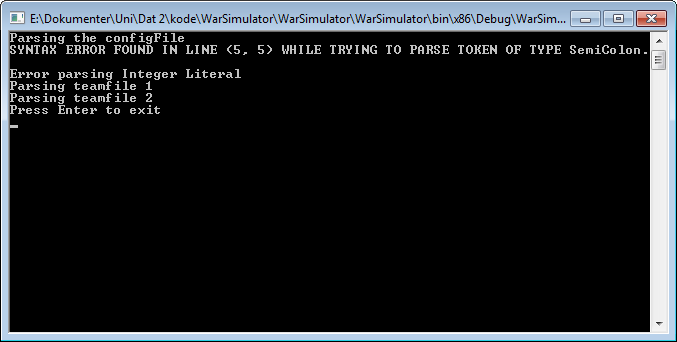
\includegraphics[scale=0.8]{rapport/7/figures/errorreporterprint}
			\caption{Printing of errors to the console}
			\label{fig:prterr}
		\end{figure}
	
	\subsection{GameDataValidator}
		The {\it GameDataValidator} class (see section \ref{sec:gdv}) prints errors to the console if it is unable to validate some of the data. 
		The error messages are very simple, which can make it difficult to find out what is wrong in the config file or team files. 
		The messages are:
		\begin{itemize}
			\item Maxima exceeded - This message is given when a UnitStat exceeds a Maxima
			\item Coordinates out of range - This message is given when a position is outside the {\it Grid}
			\item Positions overlap - This message is given when two regiments stand on the same position
		\end{itemize}
		To make debugging easier these messages could be more specific by referencing the regiment who gives the error.
		
	
		
		